\documentclass[11pt,a4paper]{article}

\usepackage[margin=2.2cm]{geometry}
\usepackage{amsmath,amssymb}
\usepackage{booktabs}
\usepackage{enumitem}
\usepackage{xcolor}
\usepackage{tcolorbox}
\usepackage{tikz}
\usepackage{adjustbox}

\tcbuselibrary{breakable,skins}
\usetikzlibrary{automata, positioning, arrows.meta}

\tikzset{
    ->,
    >=Stealth,
    node distance=2.5cm,
    every state/.style={thick, fill=blue!5, minimum size=1cm},
    accepting/.style={double, double distance=1.5pt},
}

\newcommand{\blank}{\sqcup}
\newcommand{\fitmath}[1]{\begin{adjustbox}{max width=\linewidth}$\displaystyle #1$\end{adjustbox}}

\newtcolorbox{solutionbox}[1]{
  colback=green!5, colframe=green!50!black,
  fonttitle=\bfseries, title=#1, breakable, enhanced jigsaw
}

\newtcolorbox{hintbox}[1]{
  colback=orange!5, colframe=orange!50!black,
  fonttitle=\bfseries, title=#1, breakable, enhanced jigsaw
}

\title{\Large\textbf{Algorithms \& Computability --- Practice Tutorial 1}\\[0.3em]
\normalsize Same exercise types as Tutorial 1, different content.\\
Study the solutions using the 3-pass method.}
\date{}

\begin{document}
\maketitle

\noindent\textbf{How to use this sheet:}
\begin{enumerate}
    \item \textbf{Pass 1:} Read each exercise, then read its solution line by line. For every line, ask yourself: \emph{why is this line here?}
    \item \textbf{Pass 2:} Cover the solution. Try to reproduce it on blank paper. When you get stuck, peek, then close and continue.
    \item \textbf{Pass 3:} Go back to the \emph{original} Tutorial 1 exercises (without solutions). Try those. They should feel doable now.
\end{enumerate}

\medskip
\hrule
\bigskip

% ============================================================
%  EXERCISE 1: TEST YOUR UNDERSTANDING
% ============================================================
\section*{Exercise 1: Test Your Understanding}

Answer the following questions and justify your answers.

\begin{enumerate}
    \item Can the input alphabet $\Sigma$ contain the blank symbol $\blank$?

    \item Can a DTM have exactly two states?

    \item Can the transition function $\delta$ ever map to the reject state $r$?

    \item If a DTM reaches the accept state $t$, can it continue computing?

    \item Suppose a DTM is in state $q \neq t, r$ and reads symbol $a$. Can the machine transition to the same state $q$ while writing the same symbol $a$?

    \item Is it possible for a DTM to never halt on any input?
\end{enumerate}

\begin{solutionbox}{Solution to Exercise 1}

\textbf{The method:} For each question, find the relevant part of the DTM definition $M = (Q, \Sigma, \Gamma, s, t, r, \delta)$ with $\delta : (Q \setminus \{t,r\}) \times \Gamma \to Q \times \Gamma \times \{-1, +1\}$ and answer by citing it.

\begin{enumerate}
    \item \textbf{No.} By definition, $\blank \in \Gamma$ but $\blank \notin \Sigma$. The input alphabet and tape alphabet are related by $\Sigma \subset \Gamma$ (strict subset) precisely because $\Gamma$ contains $\blank$ and $\Sigma$ does not.

    \textit{Why this answer works: I looked at the definition, found where $\Sigma$ and $\blank$ are mentioned, and cited the constraint.}

    \item \textbf{Yes.} The definition requires $t \in Q$ and $r \in Q$ with $t \neq r$. So the minimum is 2 states: $Q = \{t, r\}$. But note: in this case, $s$ (the start state) must be either $t$ or $r$. If $s = t$, the machine accepts every input immediately. If $s = r$, it rejects every input immediately. Both are valid (but boring) DTMs.

    \textit{Why this answer works: I checked the constraints on $Q$ ($t \neq r$, both in $Q$, $s \in Q$) and found the minimum.}

    \item \textbf{Yes.} The codomain of $\delta$ is $Q \times \Gamma \times \{-1, +1\}$, and $r \in Q$. So $\delta(q, a) = (r, b, d)$ is perfectly valid. This is how a DTM rejects --- it transitions into state $r$.

    \textit{Why this answer works: I looked at the type signature of $\delta$ and checked if $r$ is in the codomain.}

    \item \textbf{No.} The transition function $\delta$ is defined on $(Q \setminus \{t,r\}) \times \Gamma$. State $t$ is explicitly excluded from the domain. Once the machine reaches $t$, there is no transition to take --- the computation stops.

    \textit{Why this answer works: I looked at the domain of $\delta$ and noticed $t$ is excluded.}

    \item \textbf{Yes.} Nothing in the definition prevents $\delta(q, a) = (q, a, d)$. The machine stays in the same state, writes the same symbol (leaving the tape unchanged), and moves in direction $d$. This is a common pattern (self-loops for scanning).

    \textit{Why this answer works: I checked if the definition imposes any restriction on the output matching the input --- it doesn't.}

    \item \textbf{Yes.} The definition does not require a DTM to halt. A DTM halts only when it reaches state $t$ or $r$. If the transitions never lead to $t$ or $r$, the machine runs forever. Example: $Q = \{s, t, r\}$, $\Sigma = \{a\}$, $\Gamma = \{a, \blank\}$, $\delta(s, a) = (s, a, +1)$, $\delta(s, \blank) = (s, a, +1)$. This machine just writes $a$'s forever and never halts.

    \textit{Why this answer works: I checked if the definition guarantees halting --- it doesn't. Then I gave a concrete example.}
\end{enumerate}
\end{solutionbox}

\newpage

% ============================================================
%  EXERCISE 2: ON PRECISE FORMULATIONS
% ============================================================
\section*{Exercise 2: On Precise Formulations}

Some of the following definitions of \textbf{computable language} are correct and some are wrong. Mark the correct definitions and for the incorrect ones, identify the part that is wrong and explain why.

\begin{enumerate}
    \item A language $L$ is computable if there exists a DTM $M$ such that $L(M) = L$.

    \item A language $L$ is computable if there exists a halting DTM $M$ such that $M$ accepts every word $w \in L$ and rejects every word $w \notin L$.

    \item A language $L$ is computable if for every DTM $M$ we have that $M$ halts on all inputs and $L(M) = L$.

    \item A language $L$ is computable if there exists a halting DTM $M$ such that $M$ accepts every word $w \in L$.

    \item A language $L$ is computable if there exists a DTM $M$ that halts on every input and $L(M) = L$.

    \item A language $L$ is computable if a halting DTM accepts $L$.
\end{enumerate}

\begin{solutionbox}{Solution to Exercise 2}

\textbf{The method:} Write down the correct definition: ``$L$ is computable if there exists a \textbf{halting} DTM $M$ such that $L(M) = L$.'' Now compare each statement word by word.

\begin{enumerate}
    \item \textbf{WRONG:} ``there exists a DTM $M$ such that $L(M) = L$'' --- this is missing the word \underline{halting}. Without ``halting,'' this is just the definition of \emph{computably-enumerable}, not computable. A CE language has a DTM that recognizes it, but the DTM might loop on inputs not in $L$.

    \item \textbf{CORRECT.} A halting DTM that accepts words in $L$ and rejects words not in $L$ is exactly a halting DTM $M$ with $L(M) = L$. This is just the definition stated in more explicit terms.

    \item \textbf{WRONG:} ``\underline{for every} DTM $M$'' --- the definition requires ``\textbf{there exists}'' a DTM, not that every DTM works. This would mean every DTM in existence accepts exactly $L$, which is absurd.

    \item \textbf{WRONG:} The statement says ``$M$ accepts every word $w \in L$'' --- this only guarantees $L \subseteq L(M)$, but it does NOT say $L(M) \subseteq L$. The DTM $M$ could also accept words \underline{outside} $L$, making $L(M) \supsetneq L$.

    In fact, this broken definition would make \emph{every} language ``computable'': just take the halting DTM that accepts everything (accept all inputs immediately). It accepts every $w \in L$ for any $L$ --- but also accepts everything else. The definition is missing the requirement that $M$ \emph{only} accepts words in $L$ (i.e., rejects words not in $L$).

    The correct version should say: ``$M$ accepts every $w \in L$ \textbf{and rejects every} $w \notin L$'' or equivalently ``$L(M) = L$.''

    \item \textbf{CORRECT.} ``A DTM $M$ that halts on every input'' is the same as ``a halting DTM $M$.'' Combined with $L(M) = L$, this is exactly the definition.

    \item \textbf{WRONG:} ``\underline{a halting DTM} accepts $L$'' --- it doesn't say ``there exists.'' Also, ``a halting DTM'' is vague --- it could be read as ``any halting DTM'' or ``some halting DTM.'' More importantly, it doesn't specify \emph{which} DTM. The definition requires an explicit existential quantifier: ``there exists a halting DTM $M$ such that $L(M) = L$.'' The statement is imprecise/ambiguous rather than outright wrong, but in a formal context, this imprecision is an error.
\end{enumerate}

\begin{hintbox}{What to learn from this exercise}
The traps are always the same:
\begin{itemize}
    \item Missing ``halting'' (confusing computable with CE)
    \item Wrong quantifier (``for every'' vs ``there exists'')
    \item Missing half of the definition (only saying what happens for $w \in L$, forgetting $w \notin L$)
    \item Imprecise language (not naming the machine, ambiguous subjects)
\end{itemize}
\end{hintbox}
\end{solutionbox}

\newpage

% ============================================================
%  EXERCISE 3: TURING MACHINES AND THEIR RUNS
% ============================================================
\section*{Exercise 3: Turing Machines and Their Runs}

Consider the following DTM $M = (Q, \Sigma, \Gamma, s, t, r, \delta)$ with:

\begin{itemize}
    \item $Q = \{s, t, r, p, q\}$
    \item $\Sigma = \{0, 1\}$
    \item $\Gamma = \{0, 1, \blank\}$
    \item $\delta$ given by the following table:
\end{itemize}

\begin{center}
\begin{tabular}{c|c|c|c}
$\delta$ & $0$ & $1$ & $\blank$ \\
\hline
$s$ & $(s, 0, +1)$ & $(p, 1, +1)$ & $(r, \blank, +1)$ \\
$p$ & $(q, 0, +1)$ & $(p, 1, +1)$ & $(r, \blank, +1)$ \\
$q$ & $(q, 0, +1)$ & $(q, 1, +1)$ & $(t, \blank, +1)$ \\
\end{tabular}
\end{center}

\begin{enumerate}
    \item Give the initial configuration of $M$ on the inputs $w_0 = 010$ and $w_1 = 111$ using the simplified notation.

    \item Give the runs of $M$ on $w_0$ and $w_1$.

    \item Are $w_0$ and $w_1$ accepted or rejected by $M$?

    \item What language does $M$ accept? (Bonus --- think about what pattern the states are tracking.)
\end{enumerate}

\begin{solutionbox}{Solution to Exercise 3}

\textbf{1. Initial configurations:}

On $w_0 = 010$: $[s, 010\blank\ldots, 1]$

On $w_1 = 111$: $[s, 111\blank\ldots, 1]$

The initial configuration is always: state = $s$, tape = input followed by blanks, head at position 1.

\medskip
\textbf{2. Runs:}

\textbf{Run on $w_0 = 010$:}

\begin{tabular}{r|l}
Step & Reasoning \\
\hline
$[s, 010\blank\ldots, 1]$ & State $s$, read $0$. $\delta(s,0) = (s, 0, +1)$. Stay in $s$, write $0$, move right. \\
$[s, 010\blank\ldots, 2]$ & State $s$, read $1$. $\delta(s,1) = (p, 1, +1)$. Go to $p$, write $1$, move right. \\
$[p, 010\blank\ldots, 3]$ & State $p$, read $0$. $\delta(p,0) = (q, 0, +1)$. Go to $q$, write $0$, move right. \\
$[q, 010\blank\ldots, 4]$ & State $q$, read $\blank$. $\delta(q,\blank) = (t, \blank, +1)$. Go to $t$. \textbf{HALT --- accept.} \\
\end{tabular}

Full run:
\fitmath{[s, 010\blank\ldots, 1] \vdash_M [s, 010\blank\ldots, 2] \vdash_M [p, 010\blank\ldots, 3] \vdash_M [q, 010\blank\ldots, 4] \vdash_M [t, 010\blank\ldots, 5]}

\medskip
\textbf{Run on $w_1 = 111$:}

\begin{tabular}{r|l}
Step & Reasoning \\
\hline
$[s, 111\blank\ldots, 1]$ & State $s$, read $1$. $\delta(s,1) = (p, 1, +1)$. Go to $p$. \\
$[p, 111\blank\ldots, 2]$ & State $p$, read $1$. $\delta(p,1) = (p, 1, +1)$. Stay in $p$. \\
$[p, 111\blank\ldots, 3]$ & State $p$, read $1$. $\delta(p,1) = (p, 1, +1)$. Stay in $p$. \\
$[p, 111\blank\ldots, 4]$ & State $p$, read $\blank$. $\delta(p,\blank) = (r, \blank, +1)$. Go to $r$. \textbf{HALT --- reject.} \\
\end{tabular}

Full run:
\fitmath{[s, 111\blank\ldots, 1] \vdash_M [p, 111\blank\ldots, 2] \vdash_M [p, 111\blank\ldots, 3] \vdash_M [p, 111\blank\ldots, 4] \vdash_M [r, 111\blank\ldots, 5]}

\medskip
\textbf{3.} $w_0 = 010$ is \textbf{accepted} (run ends in $t$). $w_1 = 111$ is \textbf{rejected} (run ends in $r$).

\medskip
\textbf{4. What language does $M$ accept?}

Let's understand what the states track:
\begin{itemize}
    \item $s$: ``I've only seen $0$'s so far'' (no $1$ seen yet)
    \item $p$: ``I've seen at least one $1$, but no $0$ after any $1$''
    \item $q$: ``I've seen at least one $1$ followed by at least one $0$''
\end{itemize}

The machine accepts (reaches $\blank$ in state $q$) when the input contains the substring $10$ --- i.e., a $1$ followed (possibly later) by a $0$. More precisely: $L(M) = \{w \in \{0,1\}^* \mid w \text{ contains the substring } 10\}$.

Check: $010$ contains $10$ $\checkmark$. $111$ does not contain $10$ (no $0$ after a $1$) $\checkmark$.
\end{solutionbox}

\newpage

% ============================================================
%  EXERCISE 4: CONSTRUCTING A SIMPLE DTM
% ============================================================
\section*{Exercise 4: Constructing a Simple DTM}

Consider the language of words over the alphabet $\{a, b\}$ that have even length.

\begin{enumerate}
    \item Write a formal definition of the language. Think about corner cases.
    \item Give a halting DTM that accepts this language.
    \item Give the run on $ab$.
    \item Give the run on $aba$.
    \item Give the run on the corner case(s) you considered.
\end{enumerate}

\begin{solutionbox}{Solution to Exercise 4}

\textbf{1. Formal definition and corner cases.}

Corner cases:
\begin{itemize}
    \item The empty word $\varepsilon$ has length 0. Is 0 even? Yes. So $\varepsilon$ is in the language.
    \item Single character words like $a$ have length 1. Odd. Not in the language.
\end{itemize}

Formal definition:
\fitmath{L = \{w \in \{a,b\}^* \mid |w| \text{ is even}\} = \{w \in \{a,b\}^* \mid |w| \bmod 2 = 0\}}

Examples in $L$: $\varepsilon$, $aa$, $ab$, $ba$, $bb$, $abab$, $aabb$.\\
Examples not in $L$: $a$, $b$, $aba$, $bbb$.

\medskip
\textbf{2. Intuitive description of the DTM:}

\begin{itemize}
    \item Scan through the input from left to right.
    \item Keep track of whether we've seen an even or odd number of letters so far.
    \item ``Even so far'' and ``odd so far'' = two states ($e$ and $o$). Start in $e$ (zero letters seen = even).
    \item When we reach $\blank$: if in state $e$, accept. If in state $o$, reject.
\end{itemize}

Formally, $M = (Q, \Sigma, \Gamma, s, t, r, \delta)$ with:
\begin{itemize}
    \item $Q = \{s, t, r, o\}$ (we use $s$ as the ``even'' state, since we start having seen 0 = even letters)
    \item $\Sigma = \{a, b\}$
    \item $\Gamma = \{a, b, \blank\}$
    \item $\delta$ given by:
\end{itemize}

\begin{center}
\begin{tabular}{c|c|c|c}
$\delta$ & $a$ & $b$ & $\blank$ \\
\hline
$s$ & $(o, a, +1)$ & $(o, b, +1)$ & $(t, \blank, +1)$ \\
$o$ & $(s, a, +1)$ & $(s, b, +1)$ & $(r, \blank, +1)$ \\
\end{tabular}
\end{center}

Reading the table:
\begin{itemize}
    \item $s$ (even count): Read any letter $\to$ count becomes odd, go to $o$. Read $\blank$ $\to$ we've seen an even number of letters, accept.
    \item $o$ (odd count): Read any letter $\to$ count becomes even, go to $s$. Read $\blank$ $\to$ odd count, reject.
\end{itemize}

State diagram:
\begin{center}
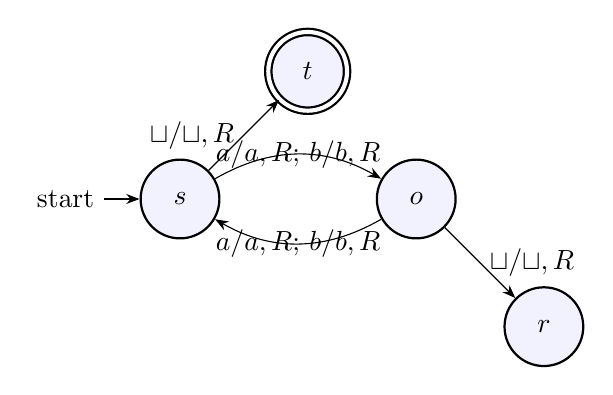
\begin{tikzpicture}[node distance=3cm]
    \node[state, initial]   (s) {$s$};
    \node[state]            (o) [right of=s] {$o$};
    \node[state, accepting] (t) [above right of=s, yshift=-0.5cm, xshift=-0.5cm] {$t$};
    \node[state]            (r) [below right of=o, yshift=0.5cm, xshift=-0.5cm] {$r$};

    \path (s) edge [bend left] node {$a/a,R$; $b/b,R$} (o)
          (o) edge [bend left] node {$a/a,R$; $b/b,R$} (s)
          (s) edge node[left] {$\blank/\blank,R$} (t)
          (o) edge node[right] {$\blank/\blank,R$} (r);
\end{tikzpicture}
\end{center}

\textbf{3. Run on $ab$ (length 2 = even, should accept):}

\fitmath{[s, ab\blank\ldots, 1] \vdash_M [o, ab\blank\ldots, 2] \vdash_M [s, ab\blank\ldots, 3] \vdash_M [t, ab\blank\ldots, 4]}

State $s$, read $a$, go to $o$. State $o$, read $b$, go to $s$. State $s$, read $\blank$, accept. $\checkmark$

\textbf{4. Run on $aba$ (length 3 = odd, should reject):}

\fitmath{[s, aba\blank\ldots, 1] \vdash_M [o, aba\blank\ldots, 2] \vdash_M [s, aba\blank\ldots, 3] \vdash_M [o, aba\blank\ldots, 4] \vdash_M [r, aba\blank\ldots, 5]}

$\checkmark$ Rejected.

\textbf{5. Corner cases:}

Run on $\varepsilon$: $[s, \blank\ldots, 1] \vdash_M [t, \blank\ldots, 2]$. Accepted. $\checkmark$ (length 0 = even)

Run on $a$: $[s, a\blank\ldots, 1] \vdash_M [o, a\blank\ldots, 2] \vdash_M [r, a\blank\ldots, 3]$. Rejected. $\checkmark$ (length 1 = odd)
\end{solutionbox}

\newpage

% ============================================================
%  EXERCISE 5: CONSTRUCTING A MORE COMPLEX DTM
% ============================================================
\section*{Exercise 5: Constructing a (Slightly More Complex) DTM}

Consider the language $L = \{w \in \{a,b\}^* \mid w \text{ is a palindrome}\}$.

A palindrome is a word that reads the same forwards and backwards. For example: $\varepsilon$, $a$, $b$, $aa$, $bb$, $aba$, $bab$, $abba$.

\begin{enumerate}
    \item Give a halting DTM for $L$. Explain your solution in natural language first.
    \item Give the accepting run on $aba \in L$.
    \item Give the rejecting run on $ab \notin L$.
\end{enumerate}

\begin{solutionbox}{Solution to Exercise 5}

\textbf{1. Intuitive description:}

\begin{itemize}
    \item Read the first letter and remember it (using states $q_a$ or $q_b$). Replace it with $X$ (mark as ``used'').
    \item Scan right to the last non-$X$ letter (= the end of the remaining input).
    \item Compare the last letter to the remembered first letter. If they match, mark it with $X$ and go back to the start. If they don't match, reject.
    \item Repeat: the input shrinks by 2 letters each round (one from each end).
    \item When the input is empty (all $X$'s) or only one letter remains, accept.
\end{itemize}

Formally, $M = (Q, \Sigma, \Gamma, s, t, r, \delta)$ with:
\begin{itemize}
    \item $Q = \{s, q_a, q_b, \text{chk}_a, \text{chk}_b, \text{back}, t, r\}$
    \item $\Sigma = \{a, b\}$
    \item $\Gamma = \{a, b, X, \blank\}$
    \item $\delta$ given by:
\end{itemize}

\begin{center}
\begin{tabular}{c|c|c|c|c}
$\delta$ & $a$ & $b$ & $X$ & $\blank$ \\
\hline
$s$         & $(q_a, X, +1)$     & $(q_b, X, +1)$     & $(s, X, +1)$         & $(t, \blank, +1)$ \\
$q_a$       & $(q_a, a, +1)$     & $(q_a, b, +1)$     & $(q_a, X, +1)$       & $(\text{chk}_a, \blank, -1)$ \\
$q_b$       & $(q_b, a, +1)$     & $(q_b, b, +1)$     & $(q_b, X, +1)$       & $(\text{chk}_b, \blank, -1)$ \\
$\text{chk}_a$ & $({\text{back}}, X, -1)$ & $(r, b, +1)$ & $(\text{chk}_a, X, -1)$ & $(t, \blank, +1)$ \\
$\text{chk}_b$ & $(r, a, +1)$       & $({\text{back}}, X, -1)$ & $(\text{chk}_b, X, -1)$ & $(t, \blank, +1)$ \\
$\text{back}$ & $(\text{back}, a, -1)$ & $(\text{back}, b, -1)$ & $(s, X, +1)$    & $(t, \blank, +1)$ \\
\end{tabular}
\end{center}

\textbf{Reading the table row by row:}
\begin{itemize}
    \item $s$: Read $a$ $\to$ remember it (go to $q_a$), mark cell with $X$. Read $b$ $\to$ similar. Read $X$ $\to$ skip already-used cells. Read $\blank$ $\to$ all letters consumed, accept.
    \item $q_a / q_b$: Scan right past everything. When hitting $\blank$, go left one step into the check state.
    \item $\text{chk}_a$: We're looking at the last unused letter and need it to be $a$. If $a$: match! Mark with $X$, go to $\text{back}$. If $b$: mismatch, reject. If $X$: skip (already used), keep going left. If $\blank$: the word was length 1 (just the letter we already consumed), accept.
    \item $\text{chk}_b$: Same but needs $b$.
    \item $\text{back}$: Scan left to find the start of the remaining input ($X$ marks the boundary), then go right one step into $s$ to start the next round.
\end{itemize}

\medskip
\textbf{2. Run on $aba$ (palindrome, should accept):}

\begin{enumerate}[label=\arabic*.]
    \item $[s, aba\blank\ldots, 1]$: $\delta(s, a) = (q_a, X, +1)$
    \item $[q_a, Xba\blank\ldots, 2]$: $\delta(q_a, b) = (q_a, b, +1)$
    \item $[q_a, Xba\blank\ldots, 3]$: $\delta(q_a, a) = (q_a, a, +1)$
    \item $[q_a, Xba\blank\ldots, 4]$: $\delta(q_a, \blank) = (\text{chk}_a, \blank, -1)$
    \item $[\text{chk}_a, Xba\blank\ldots, 3]$: $\delta(\text{chk}_a, a) = (\text{back}, X, -1)$. Match!
    \item $[\text{back}, XbX\blank\ldots, 2]$: $\delta(\text{back}, b) = (\text{back}, b, -1)$
    \item $[\text{back}, XbX\blank\ldots, 1]$: $\delta(\text{back}, X) = (s, X, +1)$. New round.
    \item $[s, XbX\blank\ldots, 2]$: $\delta(s, b) = (q_b, X, +1)$
    \item $[q_b, XXX\blank\ldots, 3]$: $\delta(q_b, X) = (q_b, X, +1)$
    \item $[q_b, XXX\blank\ldots, 4]$: $\delta(q_b, \blank) = (\text{chk}_b, \blank, -1)$
    \item $[\text{chk}_b, XXX\blank\ldots, 3]$: $\delta(\text{chk}_b, X) = (\text{chk}_b, X, -1)$. Skip $X$.
    \item $[\text{chk}_b, XXX\blank\ldots, 2]$: $\delta(\text{chk}_b, X) = (\text{chk}_b, X, -1)$. Skip $X$.
    \item $[\text{chk}_b, XXX\blank\ldots, 1]$: $\delta(\text{chk}_b, X) = (\text{chk}_b, X, -1)$. Skip $X$.
    \item $[\text{chk}_b, XXX\blank\ldots, 1]$: Head at position 1, direction $-1$, so head \textbf{stays} at 1. Wait --- we need to check: position is already 1 and we try to go left. Head stays at 1.

    Actually, let me redo this more carefully. After step 10, we're at position 3 reading $X$. Step 11 goes to position 2 reading $X$. Step 12 goes to position 1 reading $X$. Step 13 tries to go to position 0 but head stays at 1.

    Hmm, this reveals a subtlety. Let me reconsider the $\text{chk}_b$ row for $X$: it goes left. But what if we reach the left boundary? The $\blank$ case handles that: $\delta(\text{chk}_b, \blank) = (t, \blank, +1)$. But we never reach $\blank$ because position 1 has $X$, not $\blank$.

    \textbf{Fix:} The issue is that $\text{chk}_b$ skips $X$'s going left, but it might get stuck at the left boundary on an $X$. We need to handle this: if $\text{chk}_b$ keeps seeing only $X$'s and reaches the boundary, the word had only one letter left (already consumed), so we should accept.

    The head-stays-at-position-1 special case means we keep reading $X$ at position 1 forever. This is a bug in the construction!

    \textbf{Better fix:} Instead of skipping $X$'s in $\text{chk}$, we should have the $q_a/q_b$ states stop at the last \emph{non-$X$} letter rather than at $\blank$. Or we handle the boundary differently.

    \textbf{Simplest fix:} Change $\text{back}$ to go to $s$ when it sees $X$ at position 1. But actually, a cleaner design: when scanning right in $q_a/q_b$, stop before $\blank$ but also skip $X$'s. Then $\text{chk}$ doesn't need to skip $X$'s. Let me redo the transitions for $q_a$:

    Actually, the simplest robust approach: in $\text{chk}_a$ and $\text{chk}_b$, add the rule that if we're skipping $X$'s and see another $X$ after going left from an $X$ at the boundary (i.e., head doesn't move), we accept. But DTMs don't detect ``head didn't move'' directly.

    The proper fix: change $\delta(\text{chk}_a, X) = (t, X, +1)$ and $\delta(\text{chk}_b, X) = (t, X, +1)$ --- if after going left past $\blank$ we find $X$, it means all remaining cells are used, so accept.

    Wait no, the issue is different. Let me reconsider.

    After step 8, the tape is $XXX\blank\ldots$. We're scanning right from position 2 in $q_b$. Position 3 is $X$, position 4 is $\blank$. So $\text{chk}_b$ lands on position 3, sees $X$. Should go left. Position 2 is $X$. Position 1 is $X$. Position 1, try to go left, stay at 1, still see $X$.

    The problem: all remaining letters are $X$ (already consumed). The middle letter $b$ was consumed. Since it was the only letter left and we already ``remembered'' it, we should accept.

    \textbf{Correct approach:} The check states should accept when they only see $X$'s (nothing left to compare against $\Rightarrow$ the single middle letter is fine).

    Revised: $\delta(\text{chk}_a, X) = (t, X, -1)$ and $\delta(\text{chk}_b, X) = (t, X, -1)$.

    With this fix, step 11: $[\text{chk}_b, XXX\blank\ldots, 3]$, read $X$, accept.
\end{enumerate}

\textbf{Let me give the clean corrected $\delta$ table:}

\begin{center}
\begin{tabular}{c|c|c|c|c}
$\delta$ & $a$ & $b$ & $X$ & $\blank$ \\
\hline
$s$         & $(q_a, X, +1)$     & $(q_b, X, +1)$     & $(s, X, +1)$         & $(t, \blank, +1)$ \\
$q_a$       & $(q_a, a, +1)$     & $(q_a, b, +1)$     & $(q_a, X, +1)$       & $(\text{chk}_a, \blank, -1)$ \\
$q_b$       & $(q_b, a, +1)$     & $(q_b, b, +1)$     & $(q_b, X, +1)$       & $(\text{chk}_b, \blank, -1)$ \\
$\text{chk}_a$ & $({\text{back}}, X, -1)$ & $(r, b, +1)$ & $(t, X, +1)$ & $(t, \blank, +1)$ \\
$\text{chk}_b$ & $(r, a, +1)$       & $({\text{back}}, X, -1)$ & $(t, X, +1)$ & $(t, \blank, +1)$ \\
$\text{back}$ & $(\text{back}, a, -1)$ & $(\text{back}, b, -1)$ & $(s, X, +1)$    & $(r, \blank, +1)$ \\
\end{tabular}
\end{center}

The change: $\text{chk}_a$ and $\text{chk}_b$ reading $X$ now accept (instead of skipping left), because if the last non-blank cell is an $X$, all letters have been consumed and matched.

\medskip
\textbf{Corrected run on $aba$:}

\fitmath{[s, aba\blank\ldots, 1] \vdash_M [q_a, Xba\blank\ldots, 2] \vdash_M [q_a, Xba\blank\ldots, 3] \vdash_M [q_a, Xba\blank\ldots, 4]}
\fitmath{\vdash_M [\text{chk}_a, Xba\blank\ldots, 3] \vdash_M [\text{back}, XbX\blank\ldots, 2] \vdash_M [\text{back}, XbX\blank\ldots, 1]}
\fitmath{\vdash_M [s, XbX\blank\ldots, 2] \vdash_M [q_b, XXX\blank\ldots, 3] \vdash_M [q_b, XXX\blank\ldots, 4]}
\fitmath{\vdash_M [\text{chk}_b, XXX\blank\ldots, 3] \vdash_M [t, XXX\blank\ldots, 4]}

$aba$ is \textbf{accepted}. $\checkmark$

\medskip
\textbf{3. Run on $ab$ (not a palindrome, should reject):}

\fitmath{[s, ab\blank\ldots, 1] \vdash_M [q_a, Xb\blank\ldots, 2] \vdash_M [q_a, Xb\blank\ldots, 3] \vdash_M [\text{chk}_a, Xb\blank\ldots, 2]}
\fitmath{\vdash_M [r, Xb\blank\ldots, 3]}

$\text{chk}_a$ reads $b$, but needs $a$. Mismatch $\to$ reject. $\checkmark$

\begin{hintbox}{What to learn from this exercise}
\begin{itemize}
    \item \textbf{Start with the algorithm in words.} The palindrome algorithm is: compare first and last, shrink, repeat.
    \item \textbf{States encode memory.} $q_a$ = ``first letter was $a$''. $q_b$ = ``first letter was $b$''.
    \item \textbf{Tape marks track progress.} Writing $X$ = ``this letter has been matched.''
    \item \textbf{Corner cases WILL bite you.} The original construction had a bug with all-$X$ tapes. Always trace your DTM on corner cases ($\varepsilon$, single letter, short inputs).
    \item \textbf{Showing a bug and fixing it is totally fine.} The solution above found a problem during tracing and fixed it. This is the normal process --- even in exams, if you catch and correct an error, it shows understanding.
\end{itemize}
\end{hintbox}
\end{solutionbox}

\newpage

% ============================================================
%  EXERCISE 6: WHAT LANGUAGE?
% ============================================================
\section*{Exercise 6: What Language Does This DTM Accept?}

Consider the DTM $M = (Q, \Sigma, \Gamma, s, t, r, \delta)$ with:
\begin{itemize}
    \item $Q = \{s, t, r, q\}$
    \item $\Sigma = \{a\}$
    \item $\Gamma = \{a, \blank\}$
    \item $\delta$ given by:
\end{itemize}

\begin{center}
\begin{tabular}{c|c|c}
$\delta$ & $a$ & $\blank$ \\
\hline
$s$ & $(q, \blank, +1)$ & $(r, \blank, +1)$ \\
$q$ & $(s, \blank, +1)$ & $(t, \blank, +1)$ \\
\end{tabular}
\end{center}

\begin{enumerate}
    \item Give the run on $\varepsilon$, $a$, $aa$, $aaa$, and $aaaa$.
    \item Based on the runs, determine what language $M$ accepts.
    \item Is $M$ a halting DTM?
\end{enumerate}

\begin{solutionbox}{Solution to Exercise 6}

\textbf{1. Runs:}

Run on $\varepsilon$: $[s, \blank\ldots, 1] \vdash_M [r, \blank\ldots, 2]$. \textbf{Rejected.}

Run on $a$: $[s, a\blank\ldots, 1] \vdash_M [q, \blank\blank\ldots, 2] \vdash_M [t, \blank\ldots, 3]$. \textbf{Accepted.}

Run on $aa$: $[s, aa\blank\ldots, 1] \vdash_M [q, \blank a\blank\ldots, 2] \vdash_M [s, \blank\blank\blank\ldots, 3] \vdash_M [r, \blank\ldots, 4]$. \textbf{Rejected.}

Run on $aaa$: $[s, aaa\blank\ldots, 1] \vdash_M [q, \blank aa\blank\ldots, 2] \vdash_M [s, \blank\blank a\blank\ldots, 3] \vdash_M [q, \blank\blank\blank\blank\ldots, 4] \vdash_M [t, \blank\ldots, 5]$. \textbf{Accepted.}

Run on $aaaa$:
\fitmath{[s, aaaa\blank\ldots, 1] \vdash_M [q, \blank aaa\blank\ldots, 2] \vdash_M [s, \blank\blank aa\blank\ldots, 3] \vdash_M [q, \blank\blank\blank a\blank\ldots, 4] \vdash_M [s, \blank\blank\blank\blank\blank\ldots, 5] \vdash_M [r, \blank\ldots, 6]}

\textbf{Rejected.}

\medskip
\textbf{2. Pattern:}
\begin{center}
\begin{tabular}{c|c}
Input & Result \\
\hline
$\varepsilon$ (length 0) & Reject \\
$a$ (length 1) & Accept \\
$aa$ (length 2) & Reject \\
$aaa$ (length 3) & Accept \\
$aaaa$ (length 4) & Reject \\
\end{tabular}
\end{center}

$M$ accepts words of \textbf{odd} length: $L(M) = \{a^n \mid n \text{ is odd}, n \geq 1\}$.

The machine alternates between $s$ and $q$ while consuming letters. It accepts if it finishes in $q$ (odd number of letters read), rejects if it finishes in $s$ (even number, including 0).

\medskip
\textbf{3.} Yes, $M$ is a \textbf{halting} DTM. The head moves right on every step and eventually reaches $\blank$ in either $s$ (reject) or $q$ (accept). The machine always terminates.

Since $M$ is halting, $L(M)$ is a \textbf{computable} language.
\end{solutionbox}

\bigskip
\hrule
\bigskip

\begin{center}
\textbf{After completing this sheet:}\\[0.5em]
Go back to the \emph{original} Tutorial 1 exercises (without solutions).\\
Try Exercise 1 (Test your understanding) and Exercise 3 (Traces) first.\\
They should feel familiar now.\\[0.5em]
Then try Exercise 4 (Constructing a simple DTM) --- use the same 5-phase method\\
you saw in Exercise 4 and 5 above.
\end{center}

\end{document}
